\chapter{Implementierung} \label{cha:implementierung}

\section{Entwickeln einer AR-Anwendung mit Unity und AR-Foundation}

Im Folgenden ist der Entwicklungsprozess für das Implementieren eines AR-Image-Trackers mithilfe des AR-Foundation Frameworks von Unity beschrieben. Im Anschluss wird erläutert, weshalb dieser Ansatz für das Projekt obsolet wurde.

\subsection{Anlegen einer Reference-Image-Library}

% TODO: https://docs.unity3d.com/Packages/com.unity.xr.arfoundation@5.1/manual/project-setup/project-setup.html

Nachdem ein AR-Unity-Projekt nach \textit{QUELLE} angelegt wurde und das nötige Framework eingebunden wurde, stehen verschiedene Funktionen des AR-Foundation-Frameworks im Editor zur Verfügung.

Zunächst soll eine \textit{Reference-Image-Library} erstellt werden. Abbildung \ref{fig:implementierung:unity:AR-Create-Img-Lib} markiert die grundlegenden Schritte hierfür.

\begin{figure}[H]
    \centering
    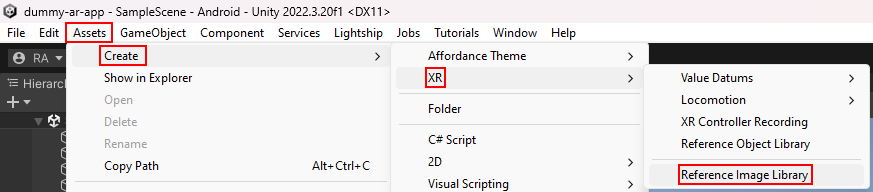
\includegraphics[width=\textwidth]{images/PrAr_UnityAR-Create-Img-Lib.png}
    \caption{Bildschirmabschnitt für das Erstellen einer Reference-Image-Library}
    \label{fig:implementierung:unity:AR-Create-Img-Lib}
\end{figure}

In der geöffneten Szene in Abbildung \ref{fig:implementierung:unity:AR-See-Img-Lib} sollte nun ein leeres Reference-Image-Library Objekt existieren.

\begin{figure}[H]
    \centering
    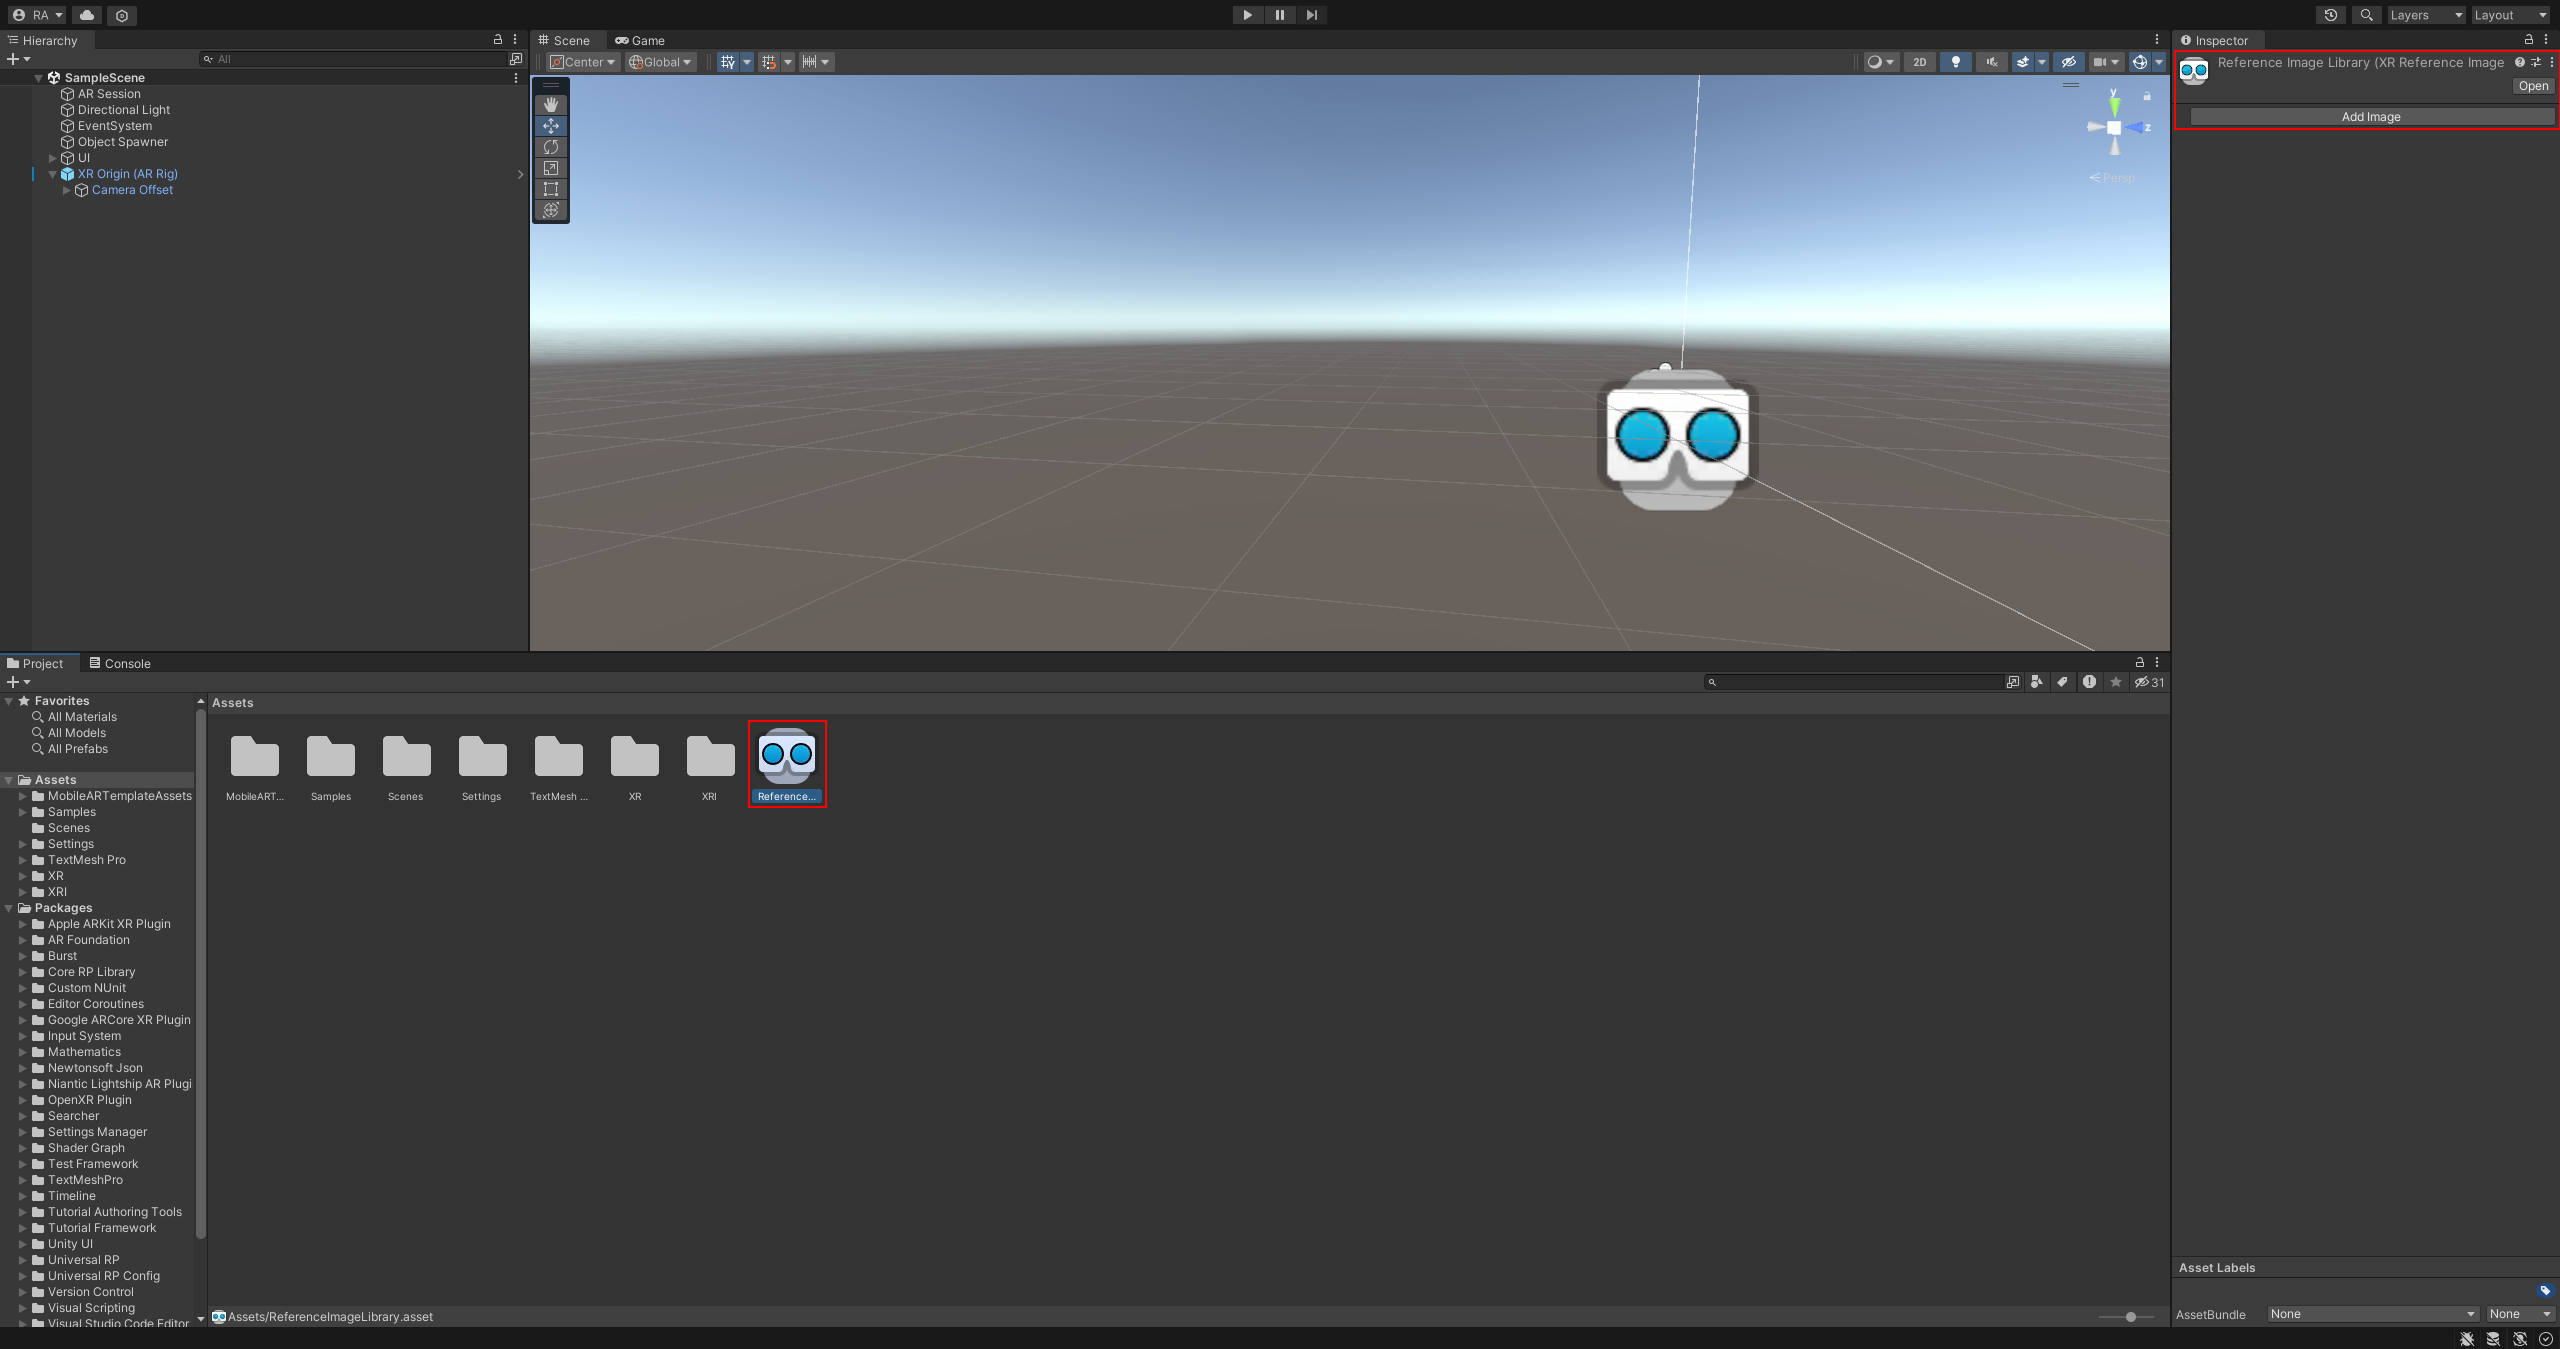
\includegraphics[width=\textwidth]{images/PrAr_UnityAR-See-Img-lib.png}
    \caption{Bildschirmabschnitt Reference-Image-Library Objekt im Editor}
    \label{fig:implementierung:unity:AR-See-Img-Lib}
\end{figure}

Die Reference-Image-Library wird benötigt, um vor der Laufzeit bereits Referenzbilder (\textit{Reference-Images}) oder Objekte zu sammeln, die von einem AR-Tracker wie etwa die Komponente \textit{XRImageTrackingSubsystem} erkannt werden können.

\subsection{Anlegen eines AR-Tracked-Image-Managers}

Die \textit{AR Tracked Image Manager} Komponente erstellt \textit{Game-Objects} für jedes gefundene Bild innerhalb des Viewports des Benutzers. Bevor ein Bild gefunden werden kann, muss die Komponente Referenz-Bilder kennen, die in der \textit{Reference-Image-Library} gespeichert sind.

Das Einbinden erfolgt, indem ein Skript an die XR-Origin Komponente angebunden wird und die dementsprechende Reference-Image-Library per Drag-and-Drop eingebunden wird. Dies aktiviert das Tracken von Bildern im AR-Raum.

\begin{figure}[H]
    \centering
    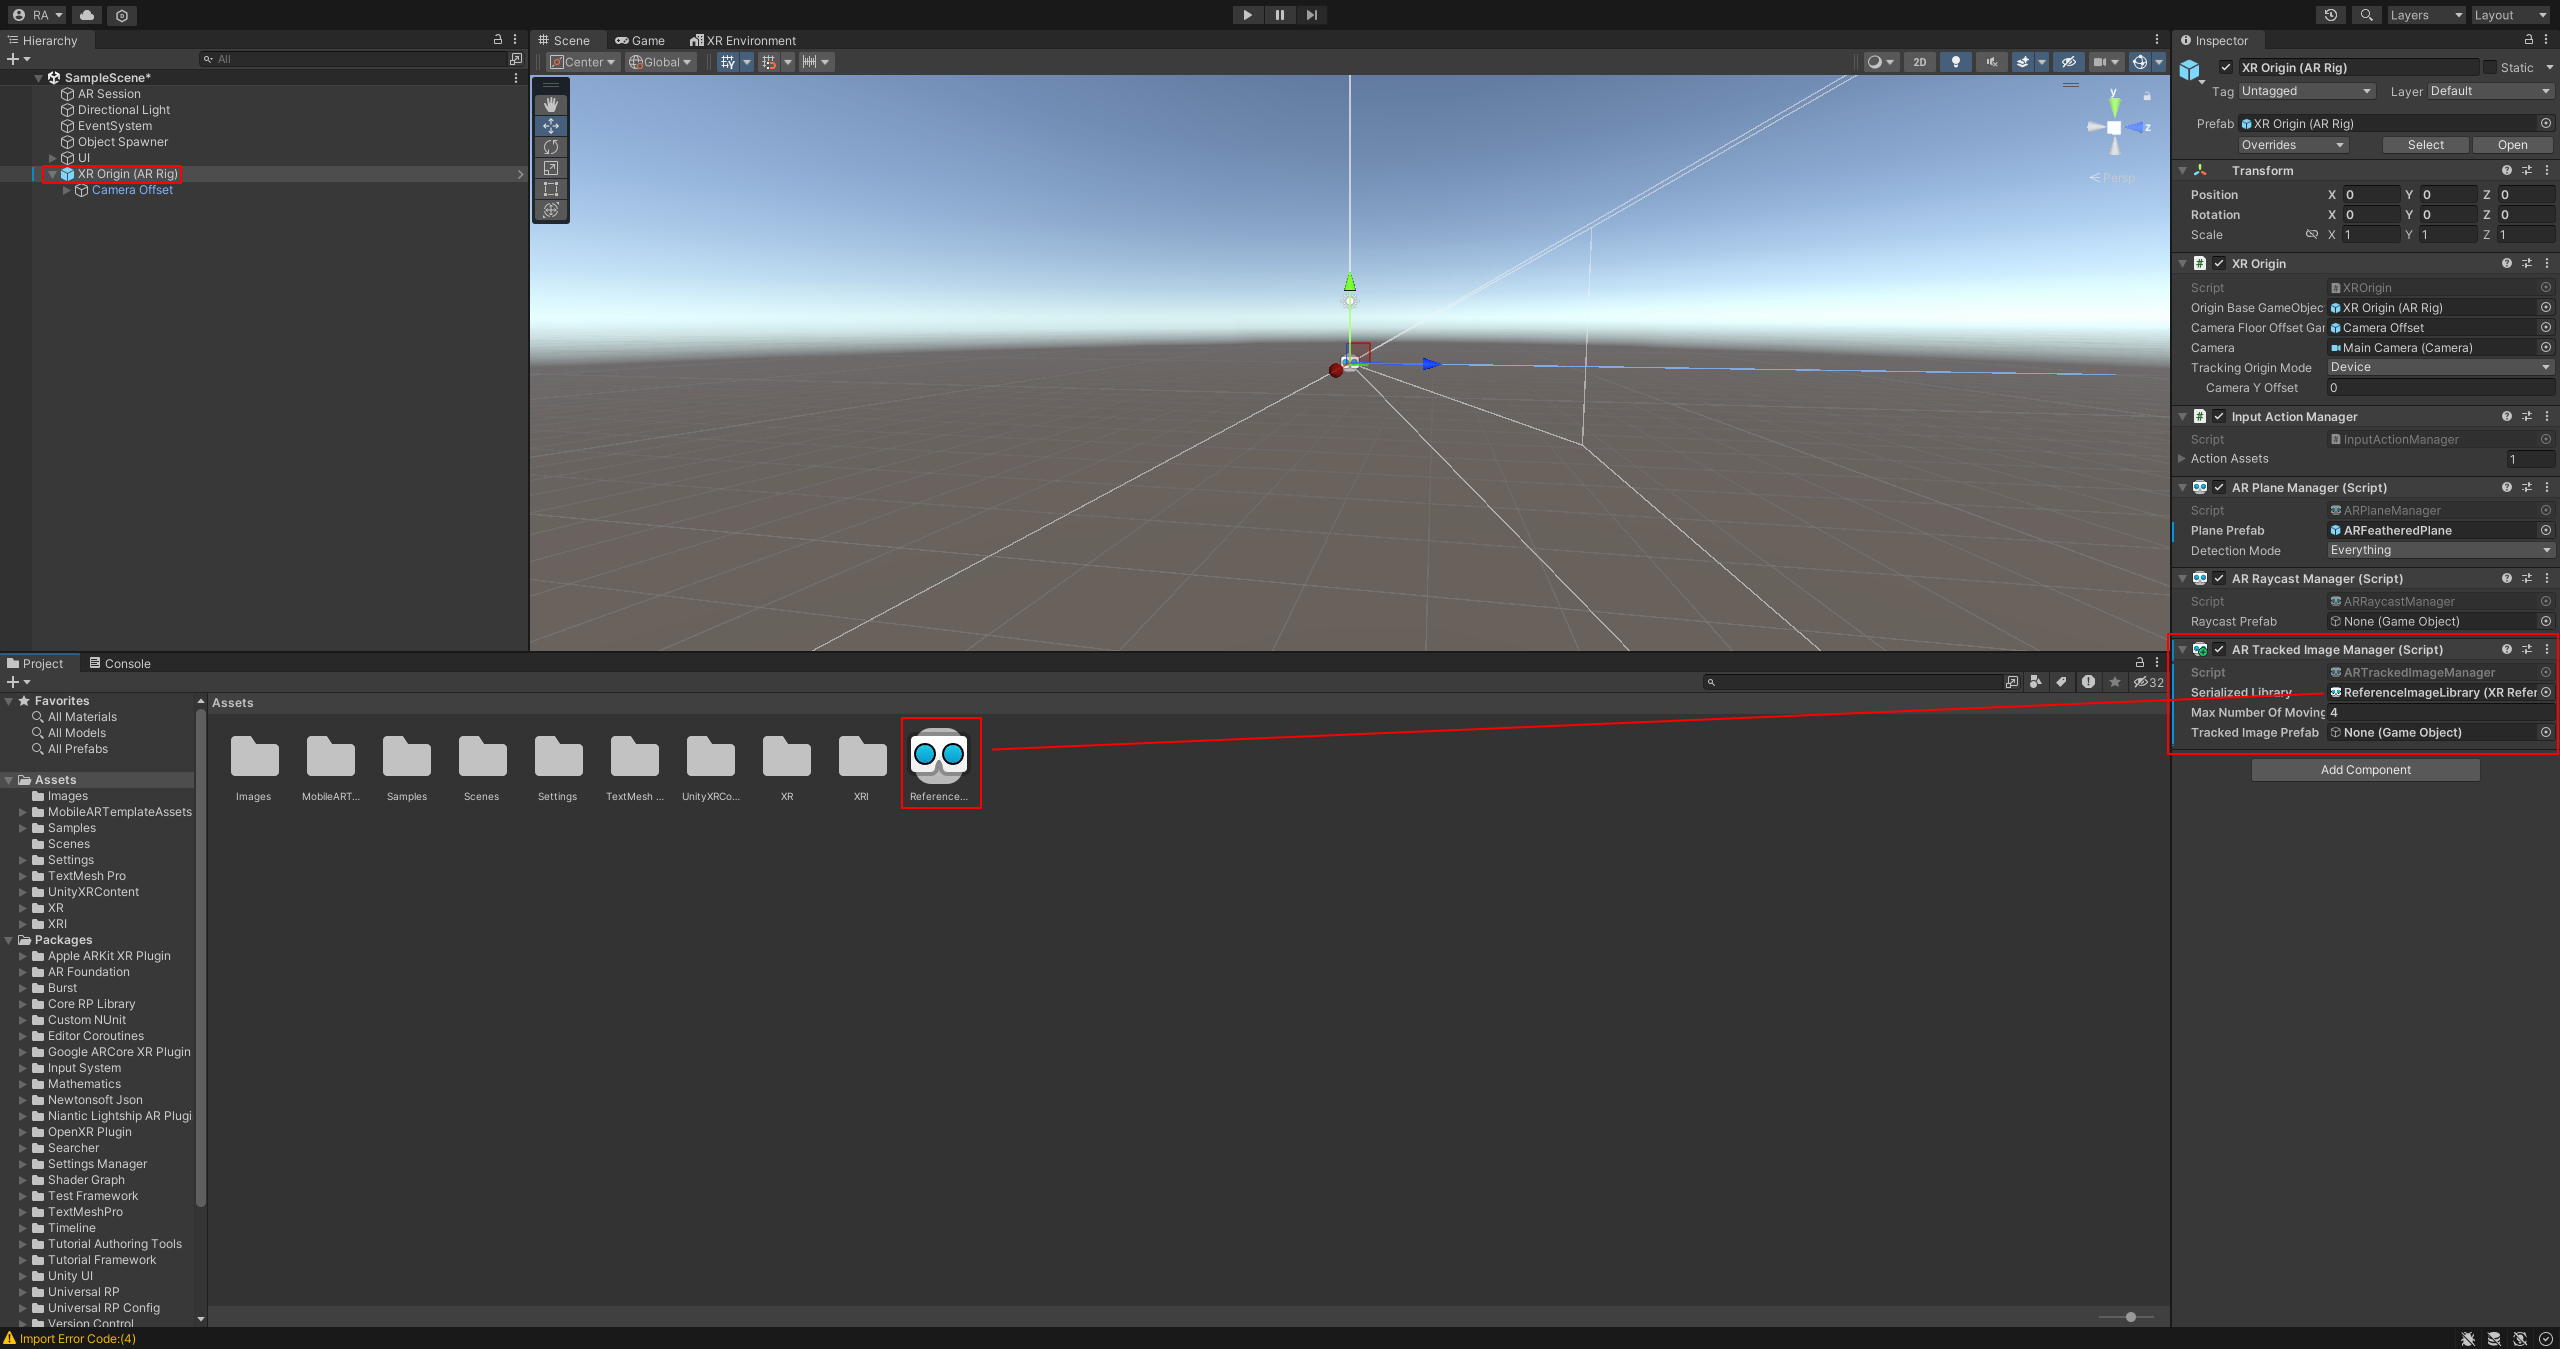
\includegraphics[width=\textwidth]{images/PrAr_UnityAR-Create-Img-Mngr.png}
    \caption{Bildschirmabschnitt für das Erstellen eines AR-Tracked-Image-Managers}
    \label{fig:implementierung:unity:AR-Create-Img-Mngr}
\end{figure}

\subsection{QR-Code-Daten aus einem Referenz-Bild lesen}

Das erkennen eines QR-Codes erfordert, dass dieser in der Reference-Image-Library bereits angelegt wurde. Nachdem dies erfolgt ist, kann der QR-Code als Textur gelesen und über einen QR-Code-Konverter wie \textit{ZXing} als Text konvertiert werden. Abbildung \ref{fig:implementierung:unity:AR-Read-Qr-Img} zeigt das erfolgreiche Umkonvertieren eines QR-Codes im AR-Raum.

\begin{figure}[H]
    \centering
    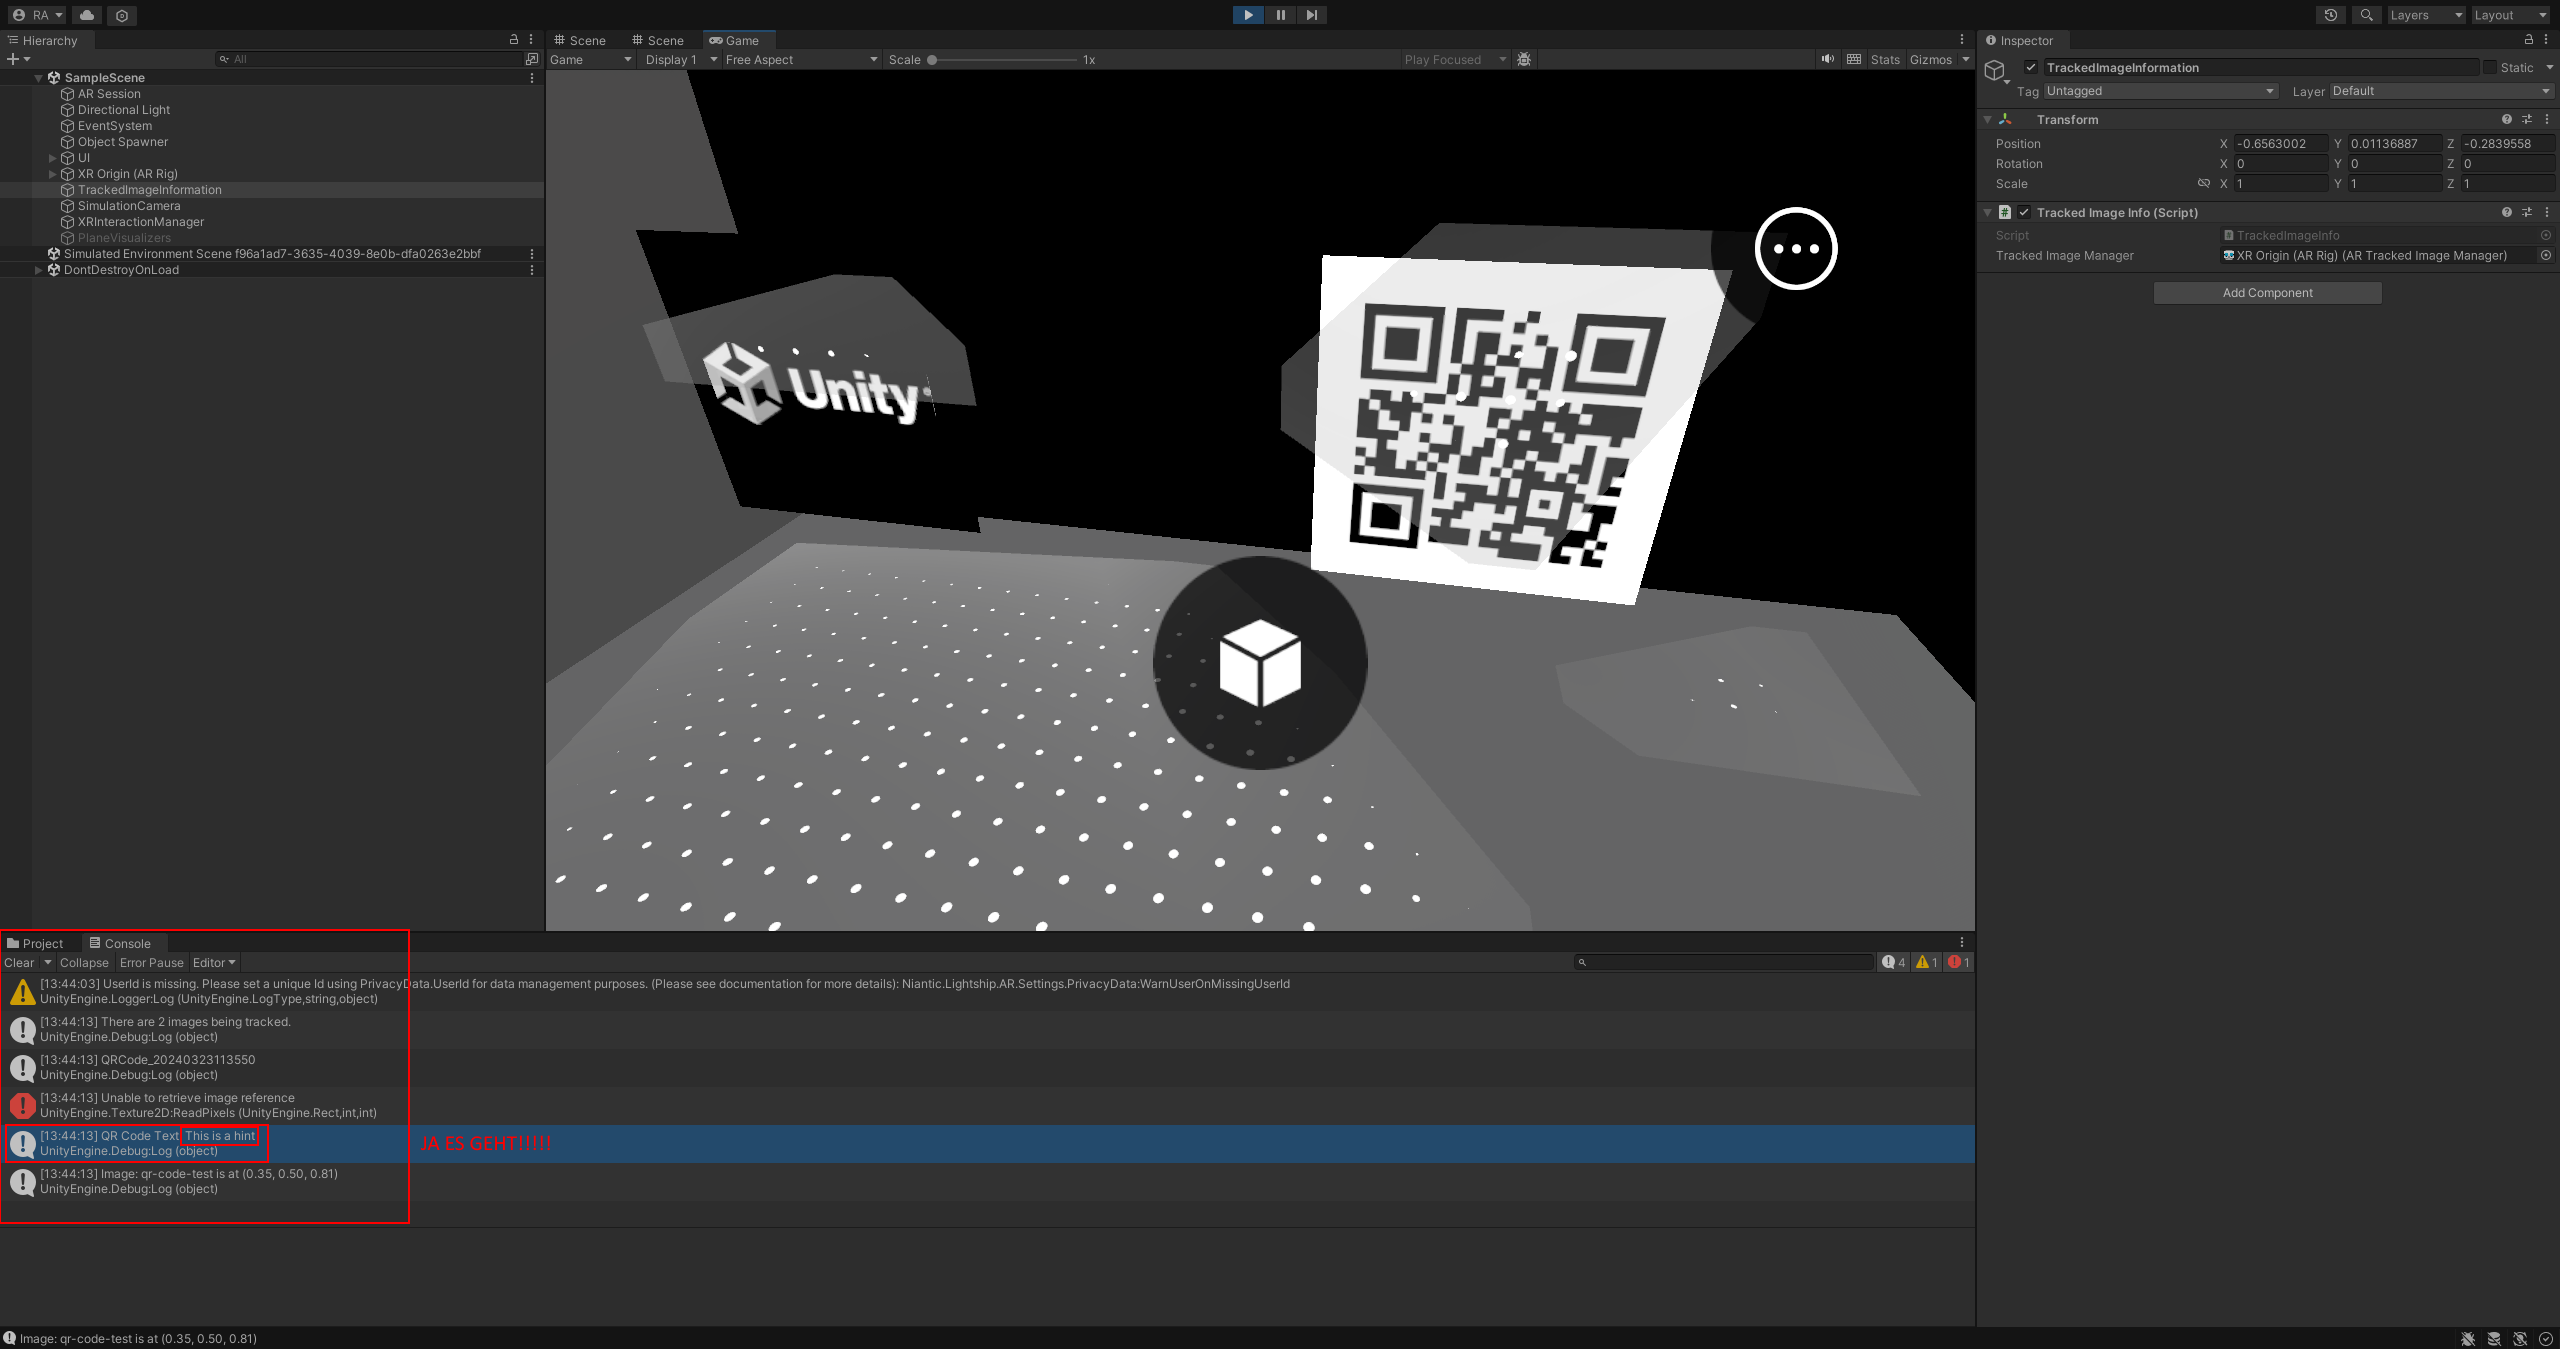
\includegraphics[width=\textwidth]{images/PrAr_UnityAR-Read-Qr-Img.png}
    \caption{Bildschirmabschnitt für das Lesen eines QR-Codes}
    \label{fig:implementierung:unity:AR-Read-Qr-Img}
\end{figure}

\subsection{Schwierigkeiten}

Leider kann über den oben beschriebenen Ansatz kein gewünschtes Ergebnis erzielt werden.

Ein Hinweistext oder -bild an der Position des QR-Codes zu platzieren, könnte theoretisch funktionieren, wie in Abbildung \ref{fig:implementierung:unity:AR-Read-Qr-Img} bereits dargestellt wird. Allerdings stellt die mangelnde Flexibilität der Reference-Image-Library ein erhebliches Hindernis für eine funktionierende Implementierung dar.

Um dieses Problem zu umgehen, müsste die Anwendung beim Start alle im System vorhandenen QR-Codes und ihre entsprechenden Lösungen über das Backend abrufen. Dies würde jedoch bei einer großen Anzahl von QR-Codes zu einer suboptimalen Benutzererfahrung führen, da die Anwendung erheblich verzögert wäre. Zusätzlich verursacht das Laden mehrerer QR-Codes einen hohen Speicheraufwand. Ein weiteres Problem besteht darin, dass die Lösungen bereits im Anwendungsspeicher geladen würden, bevor der Benutzer einen Hinweis erhalten hat. Dies könnte dazu führen, dass die Benutzer die Lösungen direkt aus dem Anwendungsspeicher extrahieren und so das Konzept der Schnitzeljagd umgehen könnten.

Diese Herausforderungen zeigen deutlich, dass Unity und AR Foundation in diesem Kontext nicht die optimale Lösung darstellen. Die genannten Einschränkungen machen es schwierig, eine flexible, effiziente und sichere Anwendung zu entwickeln, die den Anforderungen einer Schnitzeljagd entspricht. Daher ist es ratsam, alternative Technologien oder Ansätze zu berücksichtigen, die eine bessere Anpassungsfähigkeit und Sicherheit bieten.

% TODO: ALgorithmus entfernung Haversine schreiben
% TODO: Algorithmus unterscheidung characters schreiben



%\begin{lstlisting}[language=c,%
%                   caption={Überschrift des Quelltexts}]
%#include<stdio.h>
%
%int main() {
%    // Kommentar
%    int answer = 20 << 1;
%    answer += 2;
%    printf("Hallöchen Welt!\n");
%    printf("Die Antwort ist: %d\n", answer);
%    return 0;
%}
%\end{lstlisting}


%\begin{table}[htbp]
%\centering
%\begin{tabular}{|l|r|}
%\hline
%\textbf{Messwert a} & \textbf{Messwert b} \\ \hline
%9 & 5 \\ \hline
%1 & 4 \\ \hline
%1 & 3 \\ \hline
%\end{tabular}
%\caption{Überschrift der Tabelle}
%\label{tab:my-table}
%\end{table}
